\newpage
\section{モデル生物の構造およびロボット外殻の設計}
先行研究\cite{hasegawa}でモデル生物のズワイガニの解剖が行われた.
本章では,解剖によって得られた節の寸法と可動域をもとに,どのように歩脚ロボットを設計したのかを述べる.
%%%%%%%%%%%%%%%%%%%%%%%%%%%%%%%%%%%%%%%%%%%%%%%%%%%%%%%%%
\subsection{モデル生物(ズワイガニ)について}
\subsubsection{外骨格および羽状筋について}
先行研究\cite{hasegawa}で用いられた内骨格と外骨格の筋肉の付着の仕方を簡易的に示したものを図\ref{fig:naigai}に示す.
我々人間などの脊椎動物の骨のように身体の内部にあり筋肉の付着点となり,身体を支持する骨格を内骨格という.
それに対して本研究で扱う外骨格は身体を外側から覆い,体を支持し,内部を保護しつつ,筋肉の付着点となる硬い構造のことで甲殻類の外殻などが当てはまる.
外骨格は外敵からの防御にも重要な役割を果たしている反面,硬くて重い外骨格は身体の屈曲性や可動性を阻害することが多いが,甲殻類,昆虫類などは外骨格に多数の関節を持つため運動性に優れている.
しかし身体は完全に外骨格で覆われており成長が妨げられるため定期的に脱皮を行うことで身体を大きくしている.

蟹の脚の筋肉について,蟹の脚内部を充填する筋繊維の一端は節の内壁に付着し,もう一方は腱と呼ばれる組織,いわゆる蟹のすじに付着する.
腱は隣の関節の端に繋がっており,筋繊維が収縮することによって腱が引っ張られ節が開閉する.
先行研究\cite{hasegawa}でズワイガニを解剖した際に記録した長節-腕節間の腱の様子を図\ref{fig:ken}に示す.
解剖結果よりズワイガニの腱は節間膜と一体になるように挿入されていることが分かった\cite{hasegawa}.
筋繊維は腱に対して斜めに充填されており,このように配置された筋繊維を羽状筋という.
羽状筋の動きの模式図を図\ref{fig:ujo}に示す.
図\ref{fig:ujo}の左側が筋肉が伸展,右側が収縮した状態.収縮中,羽状筋の角度は27 degから41 degに増加し,腱は距離dを移動する.各筋繊維は短く太くなるが,筋全体の幅wは変化しないことを表している.
羽状筋には2つの利点があるとされている.1つ目は収縮しても膨張せず,羽状筋の角度が大きくなるだけなので限られた狭い空間で働くのに適していること,
2つ目は同じ形状と体積の平行筋と比べ収縮時に約2倍の力を発揮することが出来ることである\cite{warner1977biology}.
%%%%%%%%%%%%%%%%%%%%%%%%%%%%%%%%%%%%%%%%%%%%%%%%%%%%%%%%%
\begin{figure}[hb]
  \begin{minipage}{0.49\hsize}
    \vspace{10mm}
    \centering
    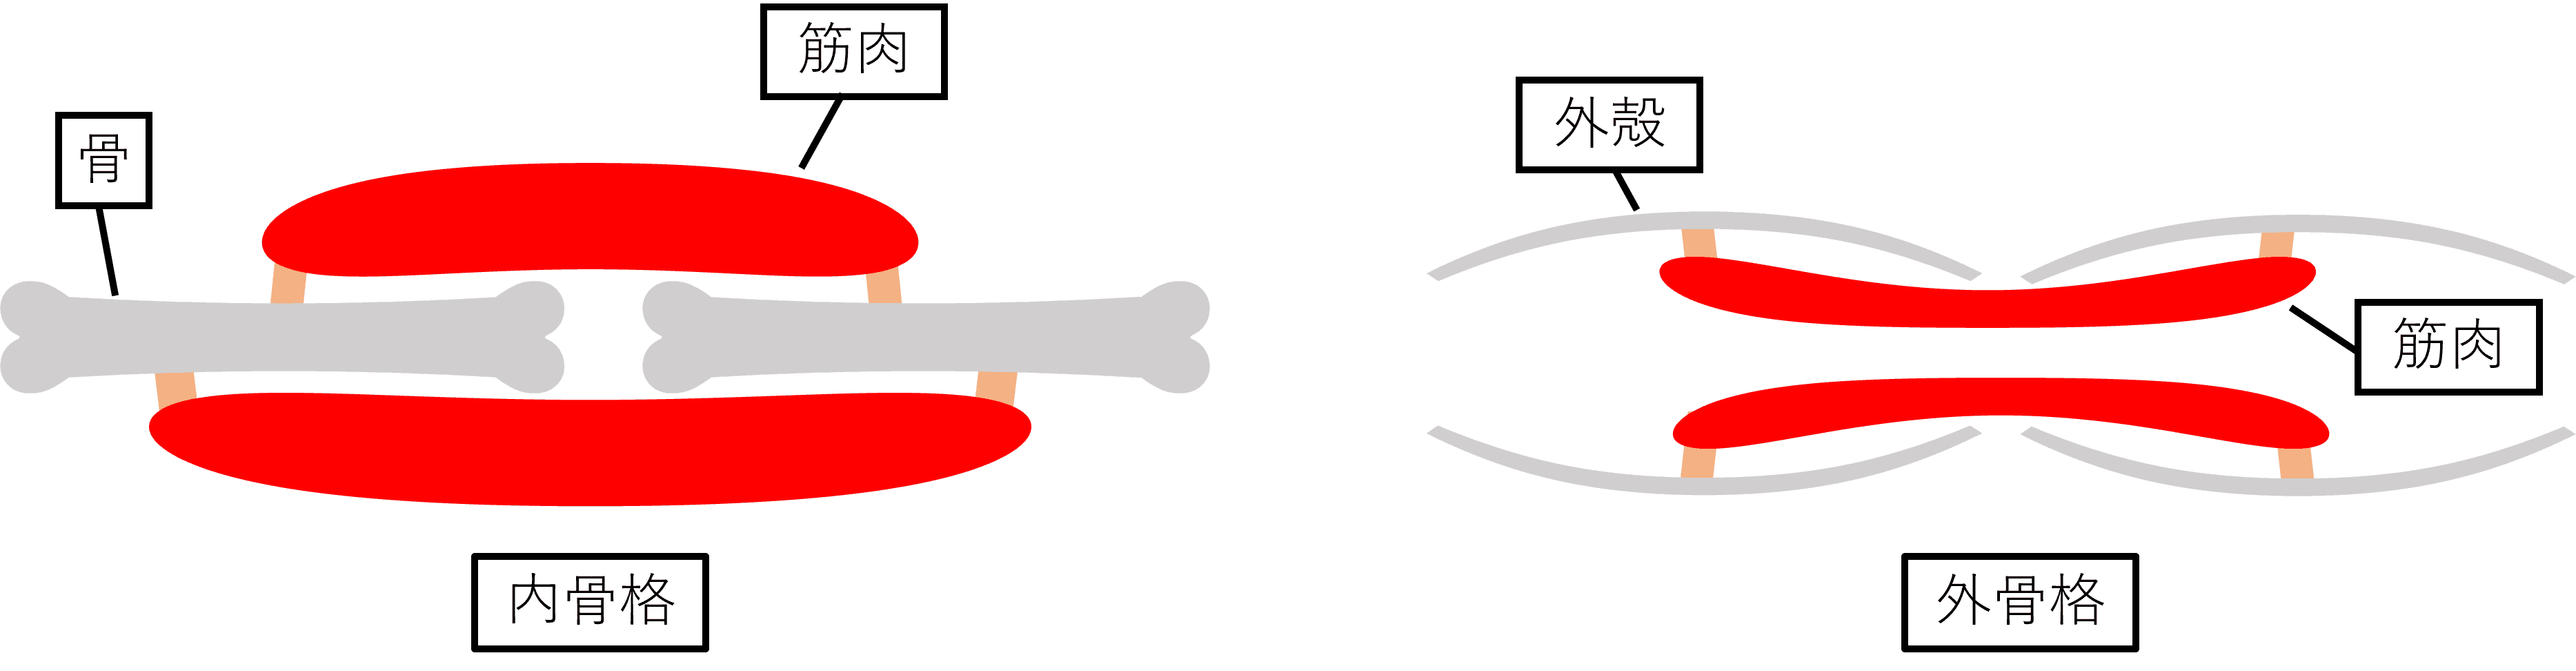
\includegraphics[scale=0.058]{image/kokkaku.png}
    \vspace{5mm}
    \caption{内骨格と外骨格\cite{hasegawa}}
    \label{fig:naigai}
  \end{minipage}
  %
  \begin{minipage}{0.49\hsize}
    \centering
    \includegraphics[scale=0.05]{image/apearance3_1.png}
    \caption{解剖に用いたズワイガニ\cite{hasegawa}}
    \label{fig:zuwai}
  \end{minipage}
\end{figure}
%%%%%%%%%%%%%%%%%%%%%%%%%%%%%%%%%%%%%%%%%%%%%%%%%%%%%%%%%
\begin{figure}[ht]
  \begin{minipage}[b]{0.39\hsize}
    \centering
    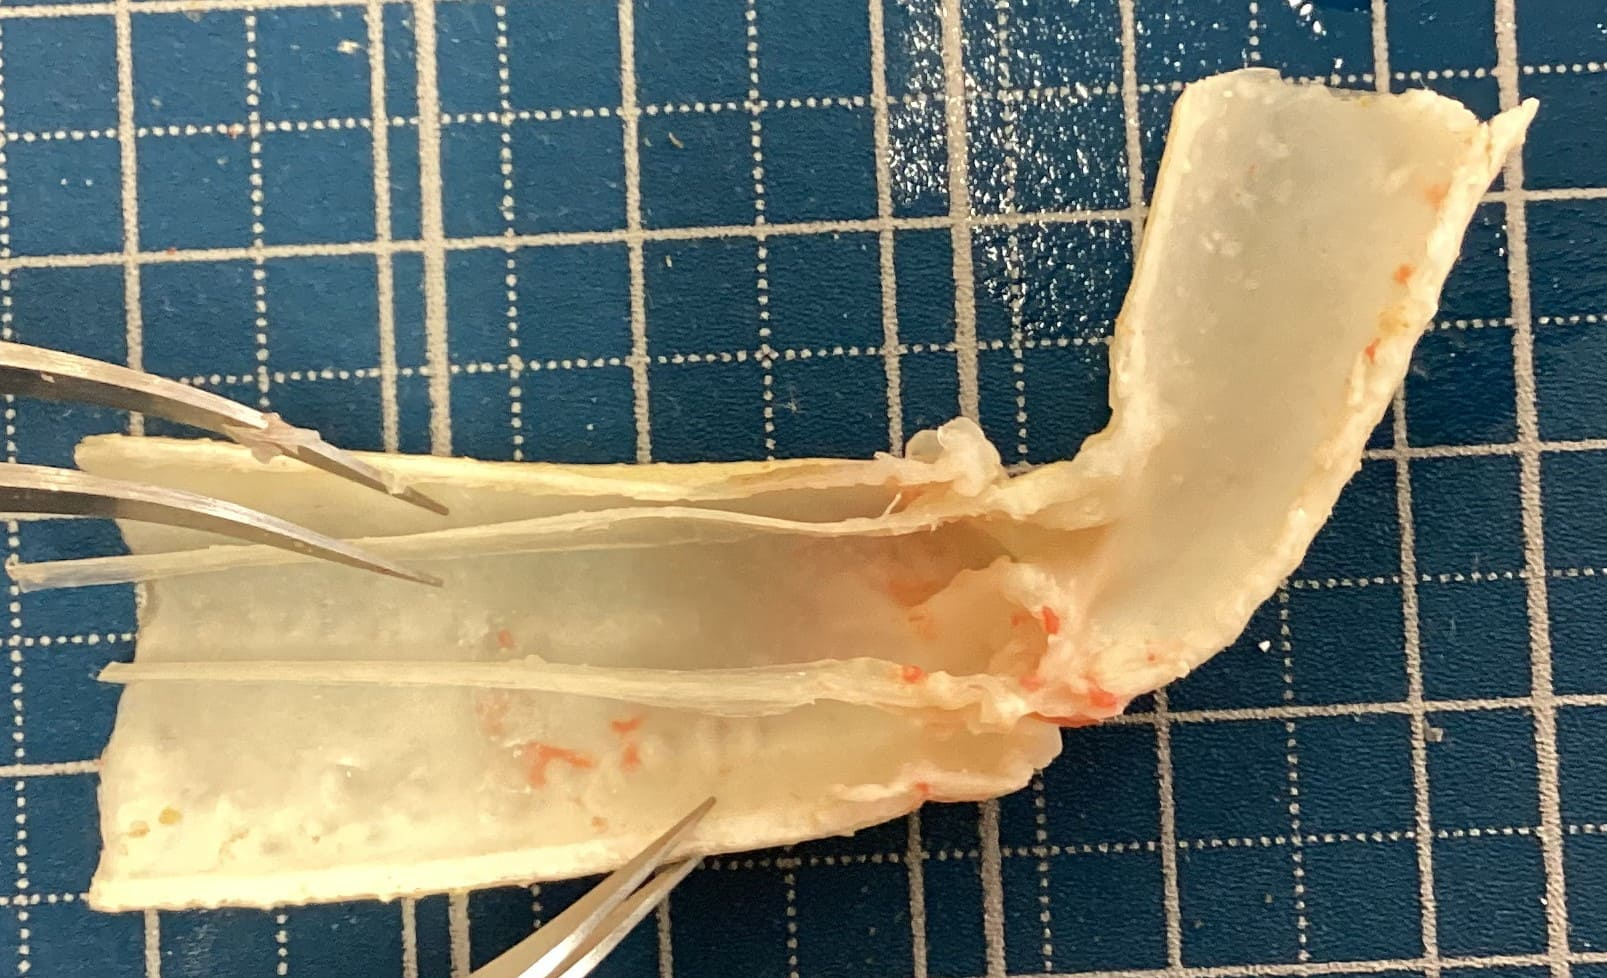
\includegraphics[scale=0.08]{image/setukanmaku.jpg}
    \caption{腱の様子\cite{hasegawa}}
    \label{fig:ken}
  \end{minipage}
  %
  \begin{minipage}[b]{0.6\hsize}
    \centering
    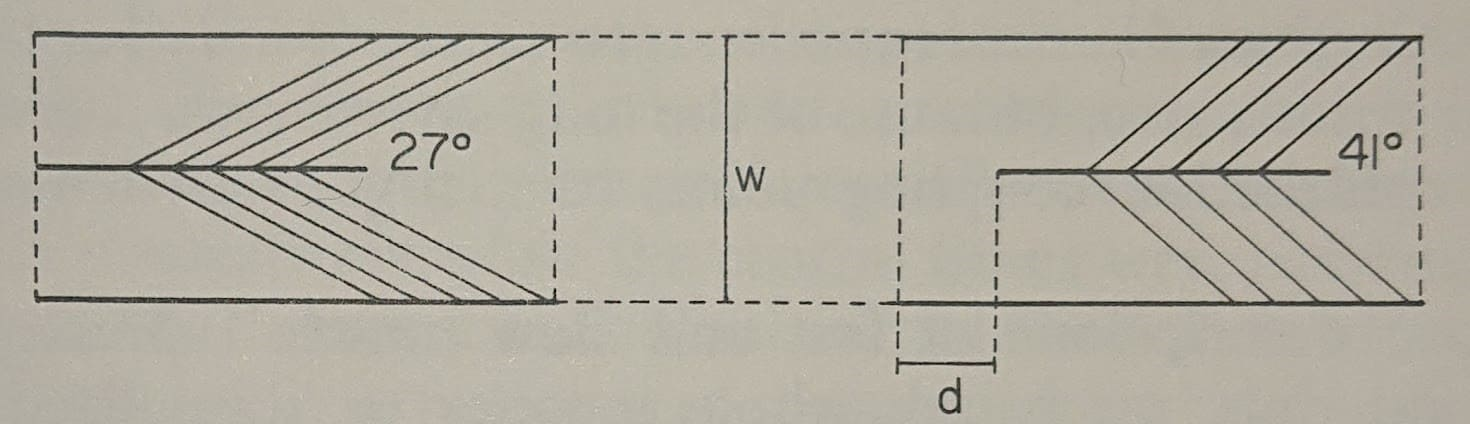
\includegraphics[scale=0.18]{image/ujo.JPG}
    \caption{羽状筋の動きを模式的に表したもの\cite{warner1977biology}}
    \label{fig:ujo}
  \end{minipage}
\end{figure}
%%%%%%%%%%%%%%%%%%%%%%%%%%%%%%%%%%%%%%%%%%%%%%%%%%%%%%%%%
\begin{figure}[!ht]
  \centering
  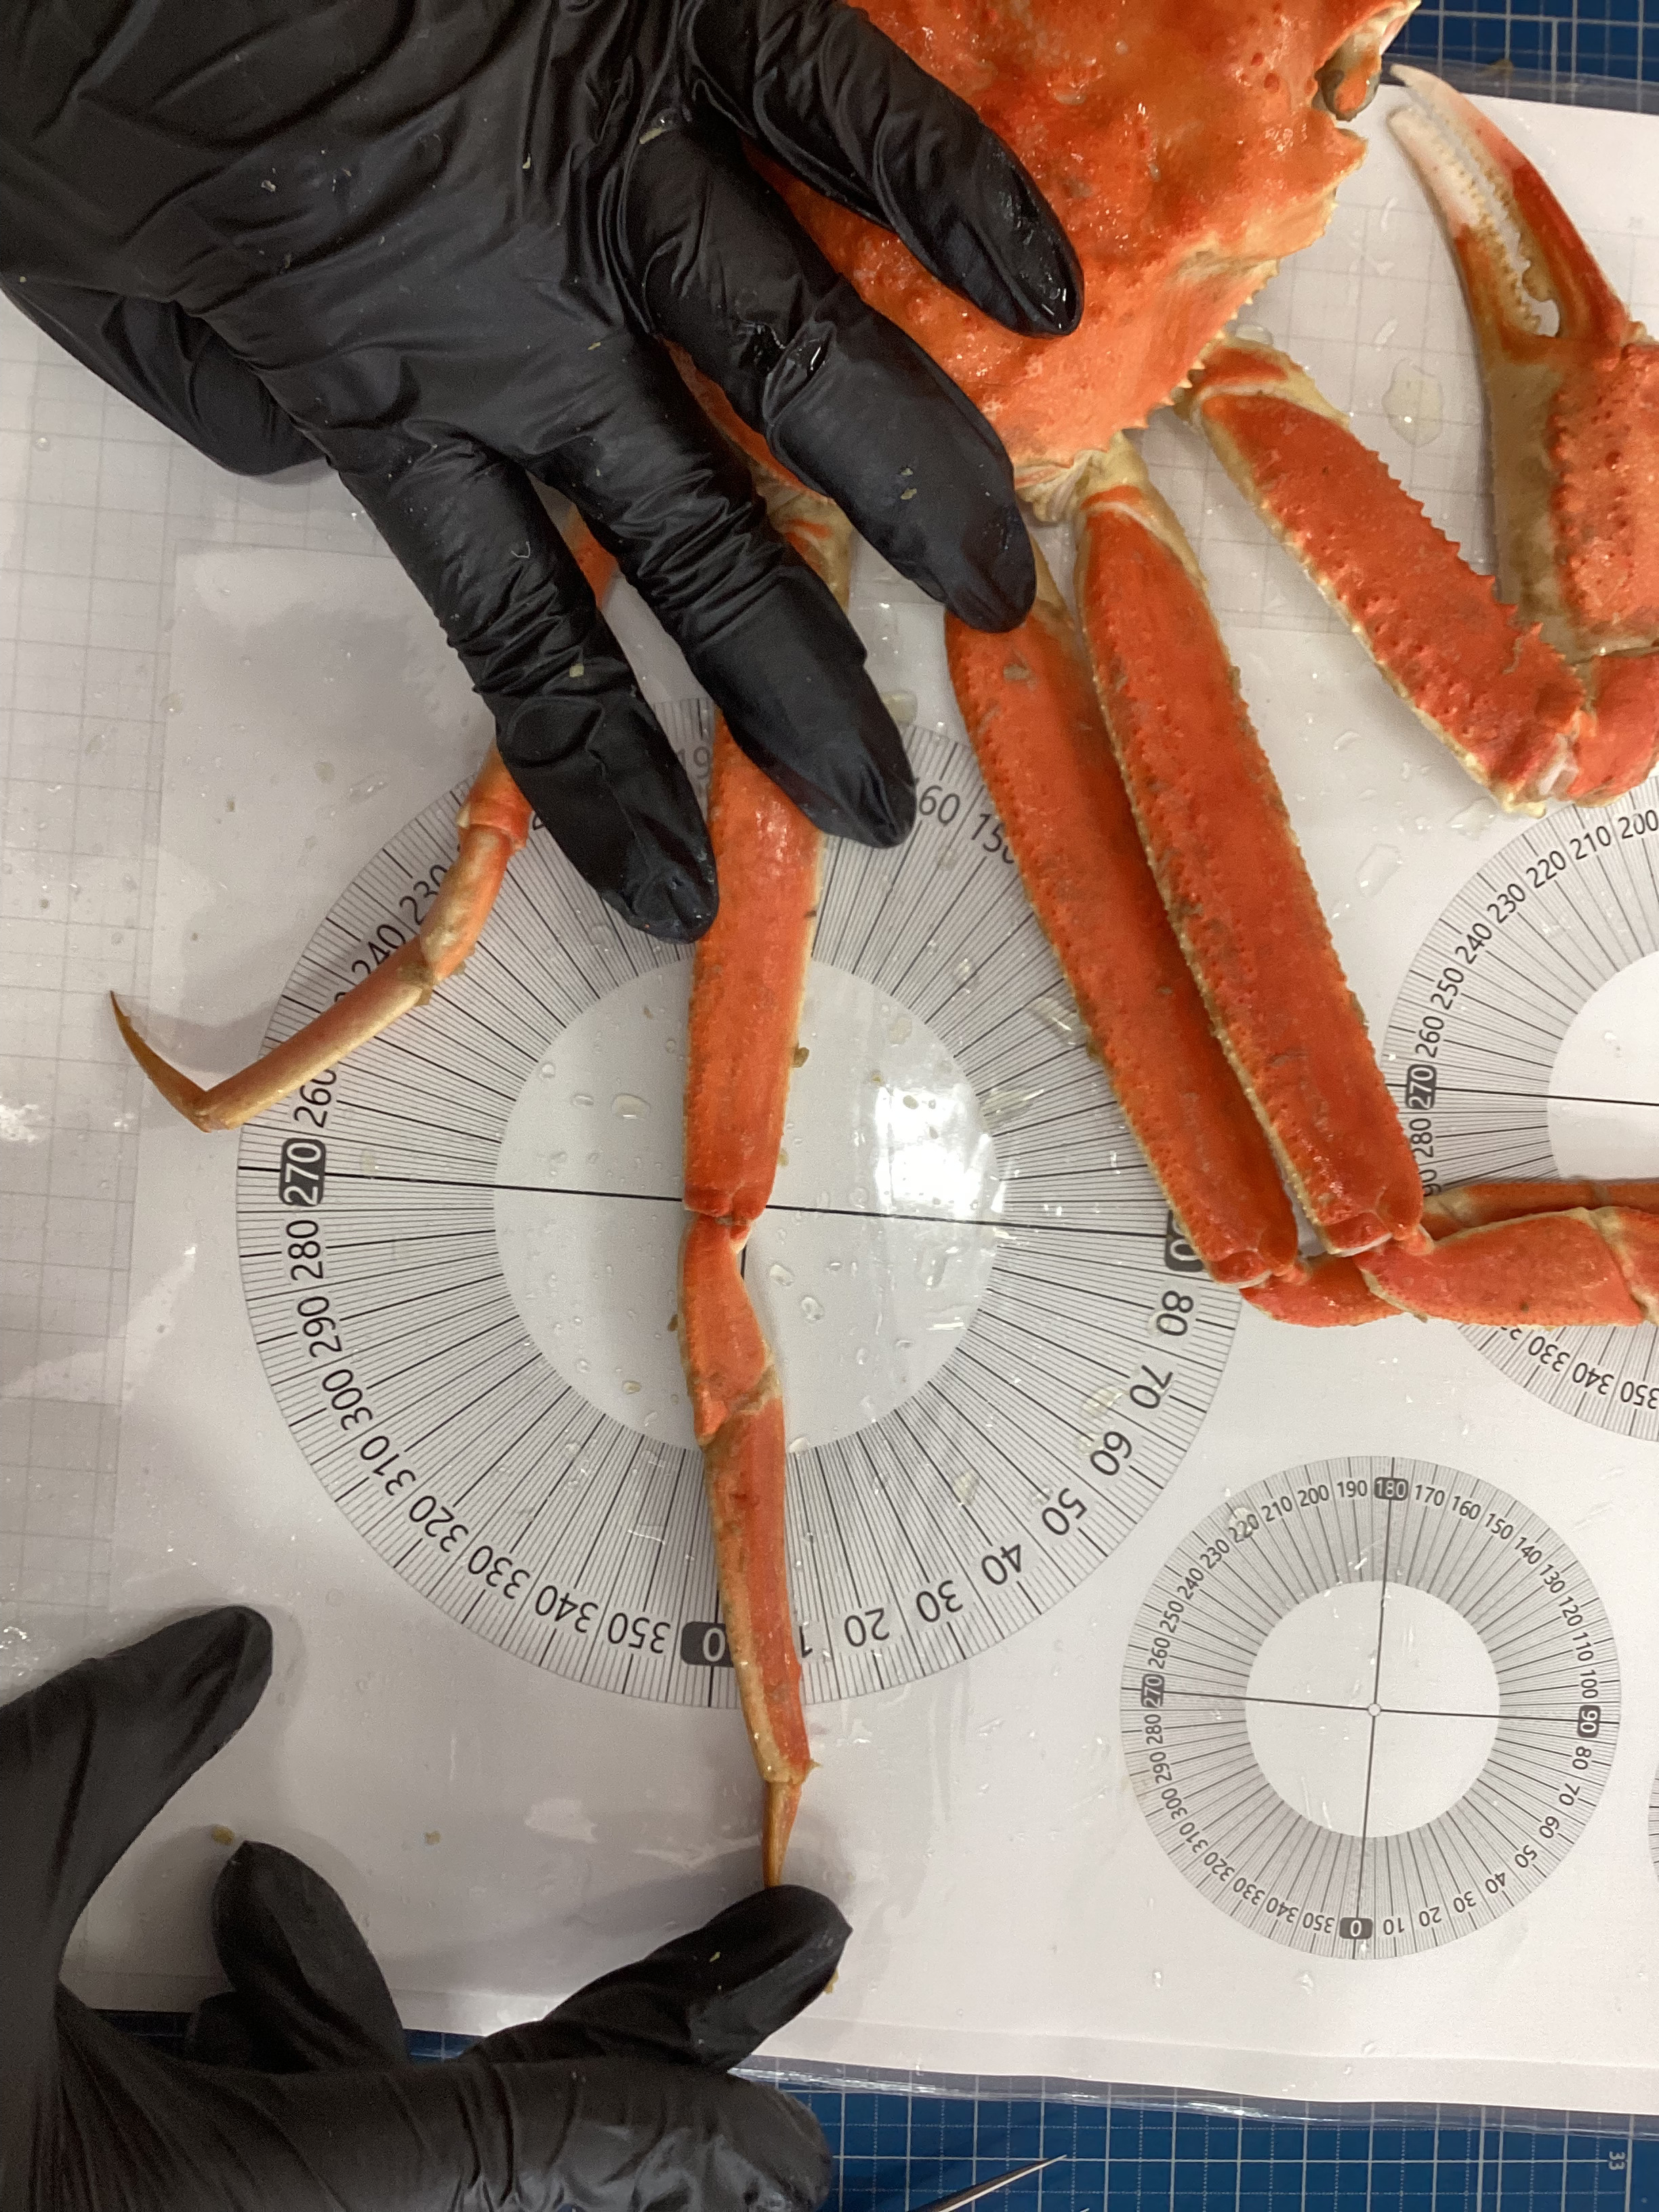
\includegraphics[scale=0.045]{image/degree_jikken.png}
  \caption{可動域の測定の様子}
  \label{fig:sokutei}
\end{figure}
%%%%%%%%%%%%%%%%%%%%%%%%%%%%%%%%%%%%%%%%%%%%%%%%%%%%%%%%%
\subsubsection{関節構造,および可動域について}
先行研究\cite{hasegawa}では実際の蟹の可動域を解剖を行い測定した.解剖には甲殻類の十脚目短尾下目ケセンガニ科のズワイガニを用いた.
測定している様子を図\ref{fig:sokutei}に示す.測定方法は,可動域を測定したい関節の軸を分度器の中心に合わせる.その時に関節の身体側の節の中心を 180°の線に合うように配置する.
そして蟹の脚で開閉動作を行い,脚先側の節の中心が閉じた状態と開いた状態での角度をそれぞれ測定してそれらを可動域とした.
なお,本研究では図\ref{fig:zuwai}中の4と書かれている下から4番目の節(第4肢)の可動域のデータを用いて機体を作製する.
第4肢の可動域を表\ref{tab:4setukadou}に示す.
%%%%%%%%%%%%%%%%%%%%%%%%%%%%%%%%%%%%%%%%%%%%%%%%%%%%%%%%%
\subsubsection{各部寸法について}
本研究で作製する歩脚ロボットは先行研究\cite{hasegawa}で行われた蟹の解剖の際に測定された寸法をもとに設計した.
測定された寸法を表\ref{tab:4setu}に示す.
なお,歩脚ロボットは外骨格内部へアクチュエータの配置が困難なことから長節,前節,指節では実測値に対して直径方向に7倍,直径方向には3.5倍,腕節は他の節より長手方向のみ5.2倍にした.
長手方向の具体的な寸法としては,長節が 350mm,腕節が 256mm,前節が 245mm,指節が 100mmである
%%%%%%%%%%%%%%%%%%%%%%%%%%%%%%%%%%%%%%%%%%%%%%%%%%%%%%%%%
\begin{table}[ht]
  \centering
  \vspace{5mm}
  \caption{第4肢の節間の可動域}
  \label{tab:4setukadou}
  \vspace{-3mm}
  \begin{tabular}{|l|c|}
  \hline
         & \multicolumn{1}{l|}{可動域 {[}deg{]}} \\ \hline
  長節-腕節間 & 0-140                            \\ \hline
  腕節-前節間 & 0-45                             \\ \hline
  前節-指節間 & 0-89                            \\ \hline
  \end{tabular}
\end{table}
%%%%%%%%%%%%%%%%%%%%%%%%%%%%%%%%%%%%%%%%%%%%%%%%%%%%%%%%% 
\begin{table}[ht]
  \centering
  \caption{第4肢の長節から指節の寸法}
  \label{tab:4setu}
  \vspace{-3mm}
  \begin{tabular}{|l|c|c|c|c|c|}
  \hline
     & \multicolumn{1}{l|}{幅-左 [mm]} & \multicolumn{1}{l|}{幅-中 [mm]} & \multicolumn{1}{l|}{幅-右 [mm]} & \multicolumn{1}{l|}{厚み [mm]} & \multicolumn{1}{l|}{長さ [mm]} \\ \hline
  長節 & 19.10                       & 21.74                       & 13.11                       & 11.05                       & 100.0                       \\ \hline
  腕節 & 10.57                       & -                           & 18.42                       & 8.74                        & 40.5                        \\ \hline
  前節 & 16.48                       & -                           & 10.40                       & 4.68                        & 70.0                        \\ \hline
  指節 & -                           & 5.60                        & -                           & 3.69                        & 30.0                        \\ \hline
  \end{tabular}
\end{table}
%%%%%%%%%%%%%%%%%%%%%%%%%%%%%%%%%%%%%%%%%%%%%%%%%%%%%%%%%
\subsection{羽状筋および関節構造のモデル化および可動域の計算}
\subsubsection{羽状筋および関節構造のモデル化}
本研究では,作製する歩脚ロボットの可動域を求めるために数理モデルを用いて計算を行った.
本研究で用いた数理モデルを図\ref{fig:model_1}に示す.数理モデルに用いた変数の説明する.
図\ref{fig:model_1}\subref{fig:model_1_before}の変数について説明する.
$\theta_f $は関節から腱への垂線と,腱の付着点から関節への直線とのなす角.
$\phi $は関節から腱への垂線と,関節から関節側にある細径MPAの交点への直線とのなす角.
$r_e $は関節から腱の付着点までの長さ.
$d_0 $は関節から腱への垂線の長さ.
$LT_e $は腱付着点から関節側にある細径MPAの交点までの長さ.
$Se_1 $は関節から腱への垂線と腱との交点から関節側にある細径MPAの交点までの長さ.
図\ref{fig:model_1}\subref{fig:model_1_after}の変数について説明する.
$\theta_e $は関節から腱への垂線と,腱の付着点から関節への直線とのなす角.
$\psi $は関節側の細径MPAの交点から腱の付着点の直線と水平な直線とのなす角.
$Se_2 $はは関節から腱への垂線と腱との交点から関節側にある細径MPAの交点までの長さ.
$d_0$ $r_e$ $LT_e$は図\ref{fig:model_1}\subref{fig:model_1_before}と同じものを表す.
図\ref{fig:model_2}\subref{fig:model_2_before}の変数について説明する.
$l_1 $は細径MPA動作前の細径MPAの長さ.
$\theta _1 $は細径MPA動作後の腱と細径MAPのなす角.
図\ref{fig:model_2}\subref{fig:model_2_after}の変数について説明する.
$l_2 $は細径MPA動作後の細径MPAの長さ.
$\theta_2 $は細径MPA動作後の腱と細径MPAのなす角.
これらの関数を用いて設計上の歩脚ロボットで必要な腱の水平方向のストロークと,収縮率 20%の細径MPAで出力可能な腱の水平方向のストロークをそれぞれ求めた.
なお
%%%%%%%%%%%%%%%%%%%%%%%%%%%%%%%%%%%%%%%%%%%%%%%%%%%%%%%%%
\begin{figure}[ht]
  %
  \begin{minipage}{0.49\hsize}
    \centering  
    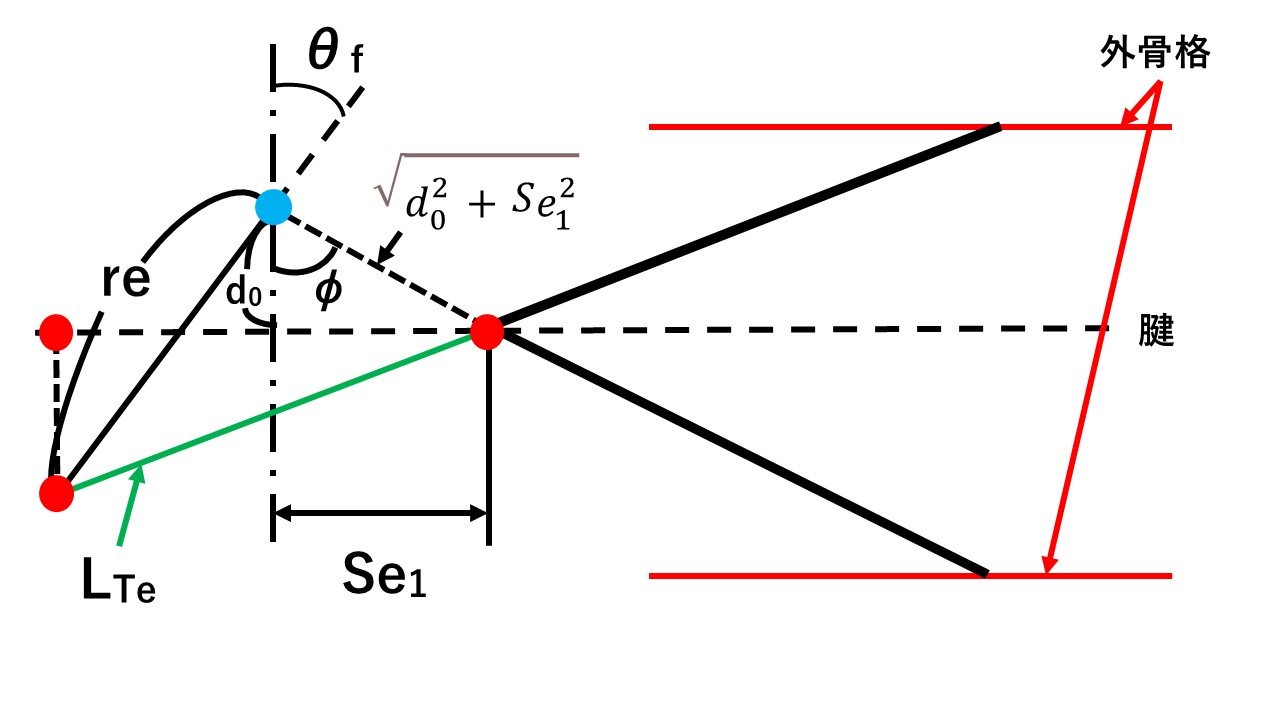
\includegraphics[scale=0.23]{image/model_1.jpg}
    \subcaption{圧縮空気印加前}
    \label{fig:model_1_before}
  \end{minipage}
  %
  \begin{minipage}{0.49\hsize}
    \centering
    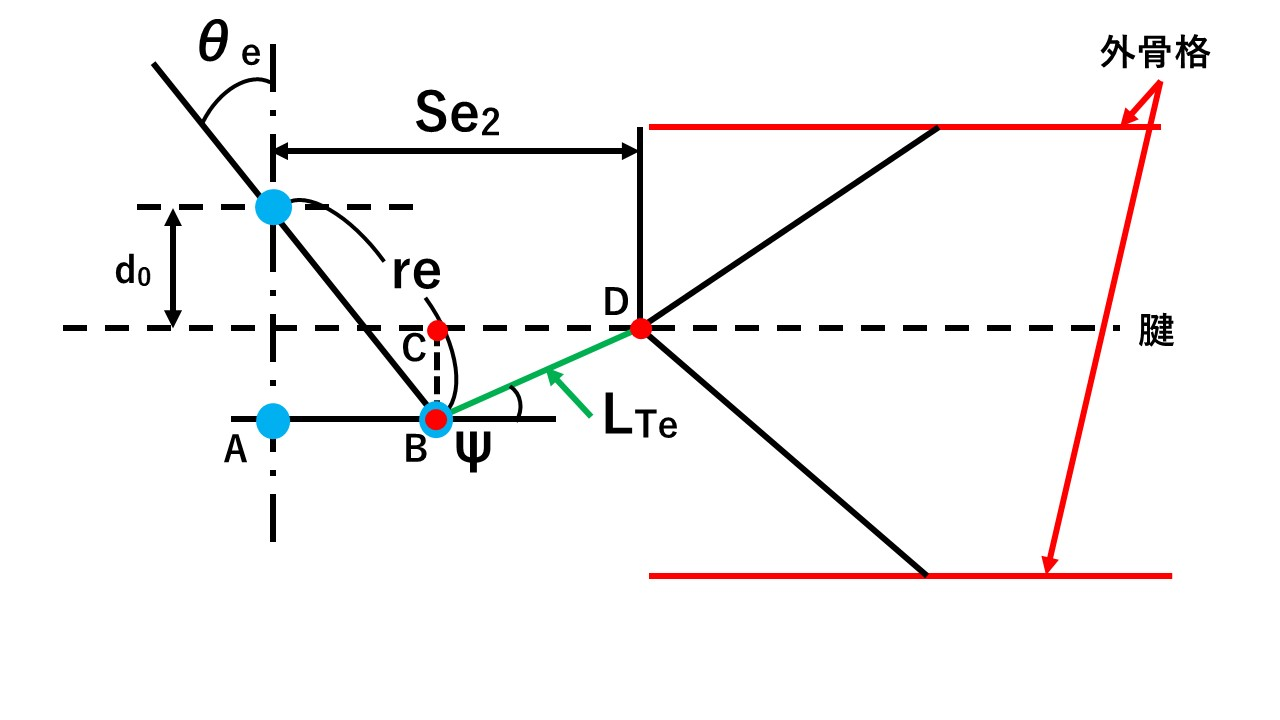
\includegraphics[scale=0.23]{image/model_2.jpg}
    \subcaption{圧縮空気印加後}
    \label{fig:model_1_after}
  \end{minipage}
  %
  \caption{可動域計算に用いた数理モデル(必要ストローク)}
  \label{fig:model_1}
\end{figure}
%
\begin{figure}[ht]
  %
  \begin{minipage}{0.49\hsize}
    \centering  
    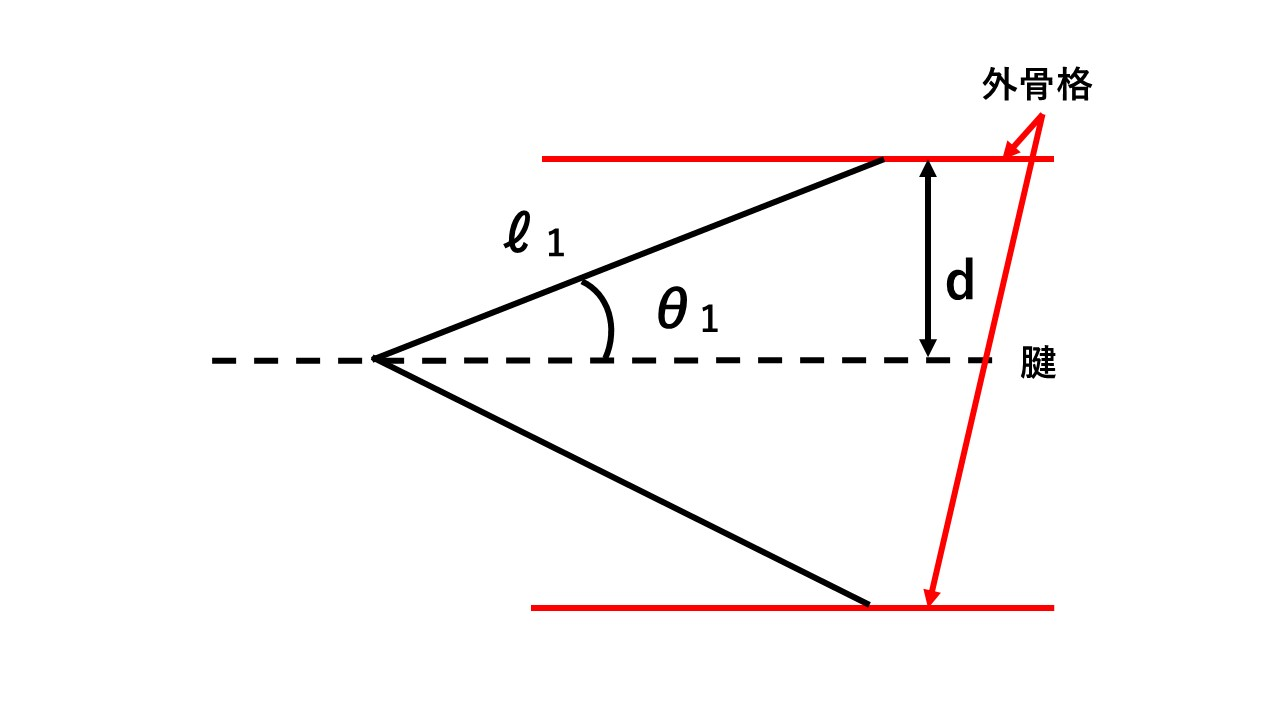
\includegraphics[scale=0.23]{image/model_2_open.jpg}
    \subcaption{圧縮空気印加前}
    \label{fig:model_2_before}
  \end{minipage}
  %
  \begin{minipage}{0.49\hsize}
    \centering
    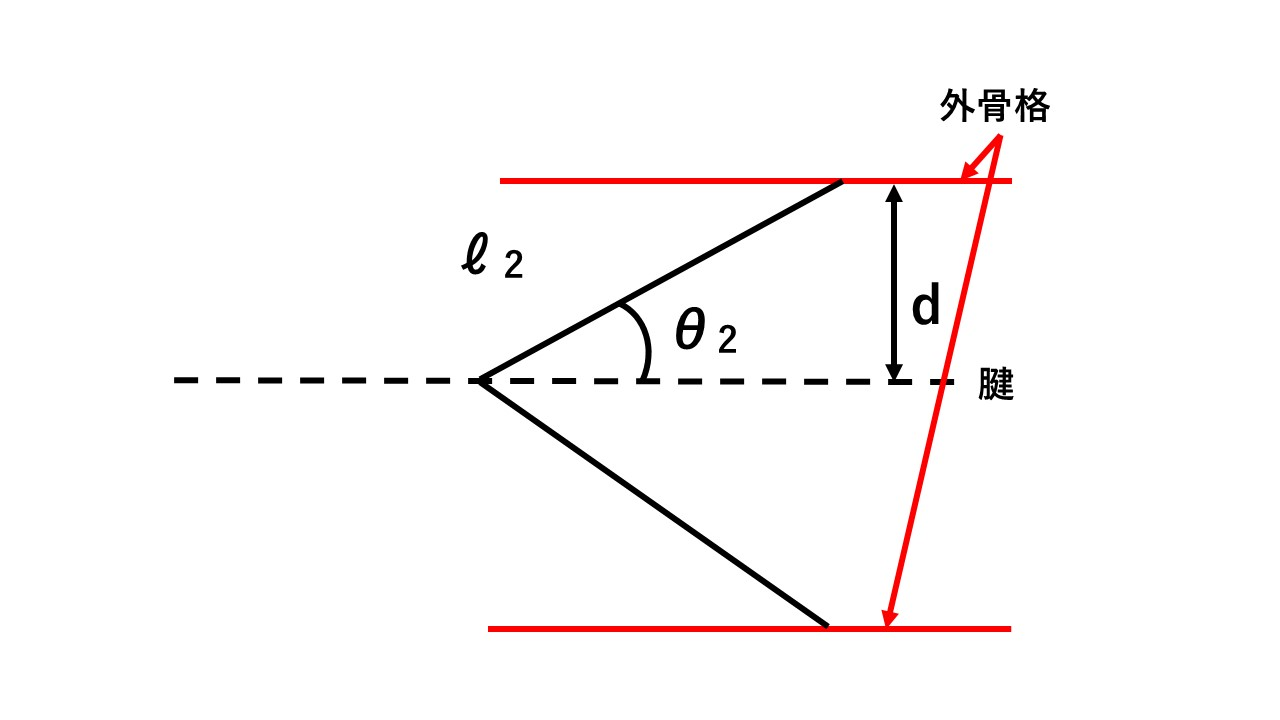
\includegraphics[scale=0.23]{image/model_2_close.jpg}
    \subcaption{圧縮空気印加後}
    \label{fig:model_2_after}
  \end{minipage}
  %
  \caption{可動域計算に用いた数理モデル(可能ストローク)}
  \label{fig:model_2}
\end{figure}
%%%%%%%%%%%%%%%%%%%%%%%%%%%%%%%%%%%%%%%%%%%%%%%%%%%%%%%%%
\subsubsection{可動域の計算}







